%! alt Parallelogram ABCD with AB = 12 and height 5, the point E on line AB beyond B with BE = 12, and E' the reflection of E in line DC. Segments BD and CE are marked equal, and the dashed segment AE' has length 26.
%! after_paragraph 1
%! scale 5/16
% The shared preamble of every Cevian figure. pipeline/figures turns these colours into theme-aware paint,
% and refuses any other colour, so draw only with them:
%   figink (lines and labels), figaux (construction lines), figaccent (the object the argument turns on),
%   figtint and figaccenttint (light fills).
\documentclass[border=1.5pt]{standalone}
\usepackage{tkz-euclide}
\definecolor{figink}{RGB}{0,0,0}
\definecolor{figaux}{RGB}{85,85,85}
\definecolor{figaccent}{RGB}{192,57,43}
\definecolor{figtint}{RGB}{221,221,221}
\definecolor{figaccenttint}{RGB}{245,213,208}
% tkz-euclide's defaults draw circles, compasses and marks in 50% grey and fill points with a tint.
\makeatletter
\def\tkz@otherlinecolor{figink}
\def\tkz@euc@circlecolor{figink}
\def\tkz@euc@compasscolor{figink}
\def\tkz@euc@mkcolor{figink}
\def\tkz@mk@fill{figink}
\def\tkz@euc@pointfillcolor{figink}
\makeatother
\tkzSetUpLine[color=figink,line width=.7pt]
\tkzSetUpArc[color=figink,line width=.7pt]
\tkzSetUpCompass[color=figink,line width=.5pt]
\tkzSetUpPoint[color=figink,fill=figink,size=3.1pt]
\tikzset{
  every picture/.style={line cap=round,line join=round,color=figink},
  circle style/.append style={color=figink,line width=.7pt},
  aux/.style={color=figaux,line width=.45pt,dash pattern=on 2.6pt off 2pt},
  key/.style={color=figaccent,line width=1pt},
  mk/.style={color=figink,line width=.5pt},
  lbl/.style={color=figink,inner sep=2.2pt},
  len/.style={color=figink,inner sep=1.5pt,font=\small},
}

\begin{document}
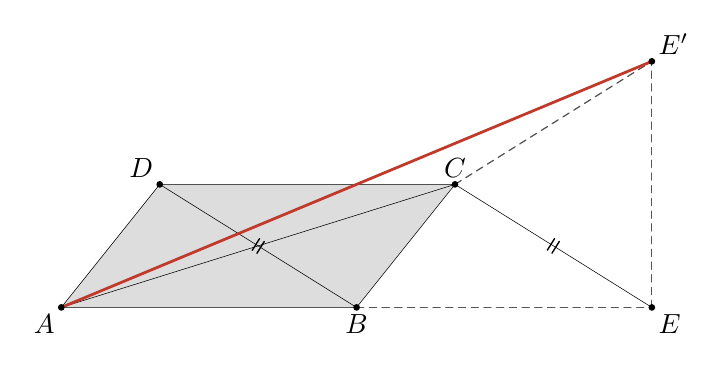
\begin{tikzpicture}
\tkzDefPoint(0.0,0.0){A} %! A = (0, 0)
\tkzDefPoint(3.7500000,0.0){B} %! B = (12, 0)
\tkzDefPoint(7.5000000,0.0){E} %! E = (24, 0)
\tkzDefPoint(1.2500000,1.5625000){D} %! D = (4, 5)
\tkzDefPoint(5.0000000,1.5625000){C} %! C = (16, 5)
\tkzDefPoint(7.5000000,3.1250000){F} %! F = reflect(E, D, C)
%! fact dist(A, B) == 12
%! fact dist(B, E) == 12
%! fact collinear(A, B, E)
%! fact area(A, B, C, D) == 60
%! fact parallel(B, D, E, C)
%! fact equal(dist(B, D), dist(C, E))
%! fact equal(dist(C, E), dist(C, F))
%! fact dist(A, F) == 26
\tkzFillPolygon[color=figtint](A,B,C,D)
\tkzDrawPolygon(A,B,C,D)
\tkzDrawSegment[aux](B,E)
\tkzDrawSegment(B,D)
\tkzDrawSegment(A,C)
\tkzDrawSegment(C,E)
\tkzDrawSegment[aux](C,F)
\tkzDrawSegment[aux](E,F)
\tkzDrawSegment[key](A,F)
\tkzMarkSegments[mark=||,size=2.5pt,mk](B,D C,E)
\tkzDrawPoints(A,B,C,D,E,F)
\tkzLabelPoint[below left,lbl](A){$A$}
\tkzLabelPoint[below,lbl](B){$B$}
\tkzLabelPoint[below right,lbl](E){$E$}
\tkzLabelPoint[above left,lbl](D){$D$}
\tkzLabelPoint[above,lbl](C){$C$}
\tkzLabelPoint[above right,lbl](F){$E'$}
\end{tikzpicture}
\end{document}
